\chapter{Desenvolvimento}

\section{Diagrama de casos de uso}
\begin{figure}[H]
	\centering
		\caption{Diagrama de casos de uso.}
		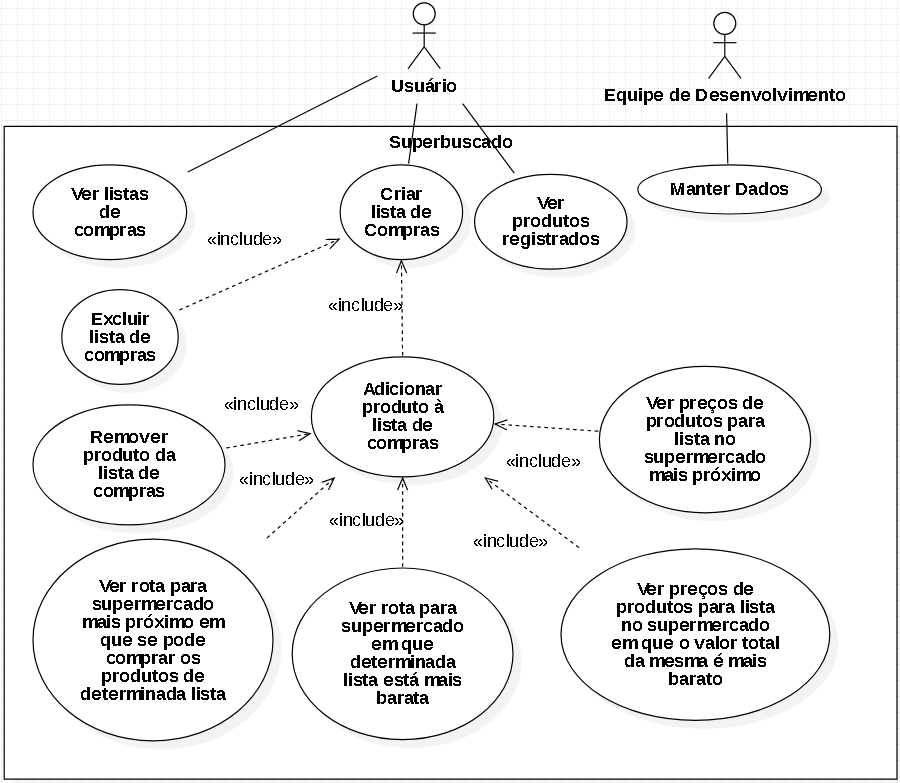
\includegraphics[scale=0.4]{Imagens/DiagramaDeCasosDeUso.png}
		\fonte{Do autor - 2019.}	
\end{figure}


\section{Especificações de caso de uso}
As  atividades que podem ser realizadas no aplicativo e os atores participantes destas, estão descritas nas sequências de imagens abaixo, figura  \ref{fig:UC001} até \ref{fig:UC010}.
\begin{figure}[H]
    \centering
        \caption{UC001.}
        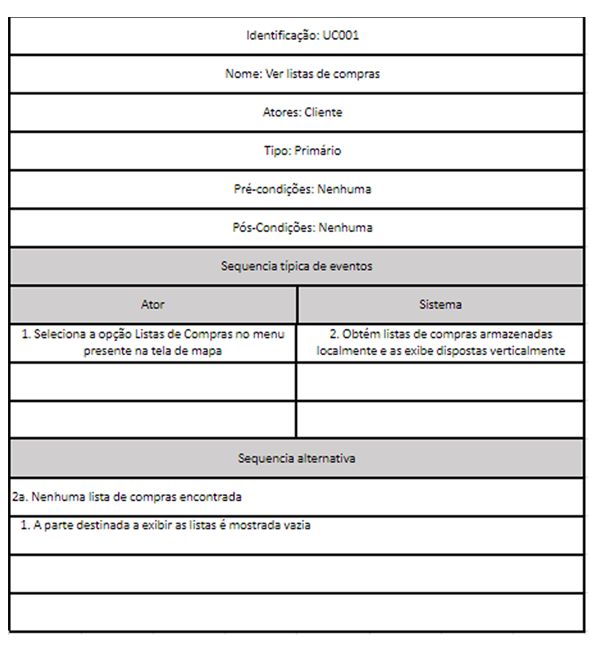
\includegraphics[scale=0.8]{Imagens/UC001.PNG}
        \fonte{Do autor - 2019.}
        \label{fig:UC001}
\end{figure}
	
\begin{figure}[H]
	\centering
		\caption{UC002}
		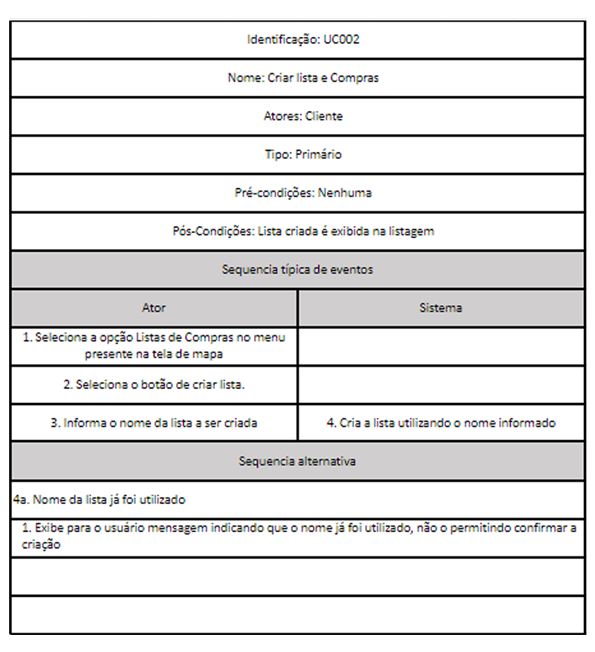
\includegraphics[scale=0.8]{Imagens/UC002.PNG}
		\fonte{Do autor - 2019.}
\end{figure}
	
\begin{figure}[H]
	\centering
		\caption{UC003}
		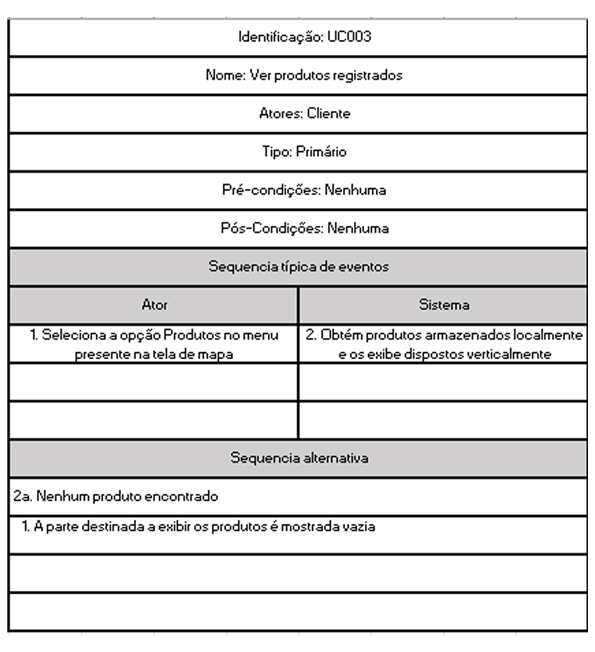
\includegraphics[scale=0.8]{Imagens/UC003.PNG}
		\fonte{Do autor - 2019.}
\end{figure}

\begin{figure}[H]
	\centering
		\caption{UC004}
		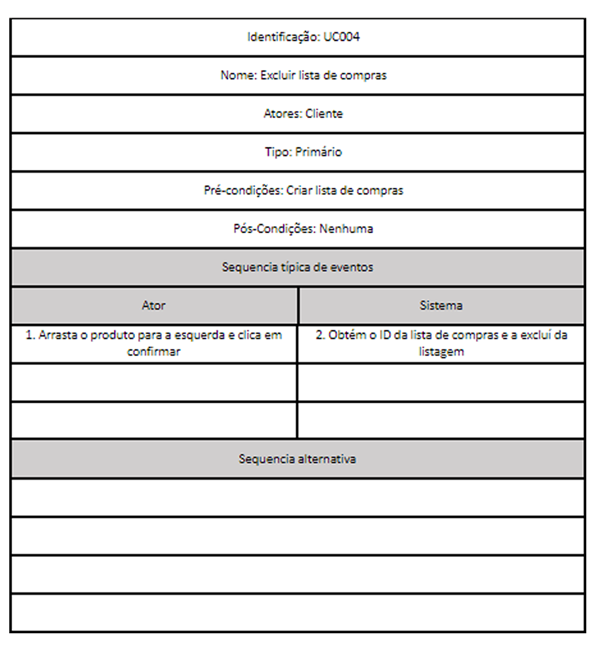
\includegraphics[scale=0.8]{Imagens/UC004.PNG}
		\fonte{Do autor - 2019.}
\end{figure}
	
\begin{figure}[H]
	\centering
		\caption{UC005}
		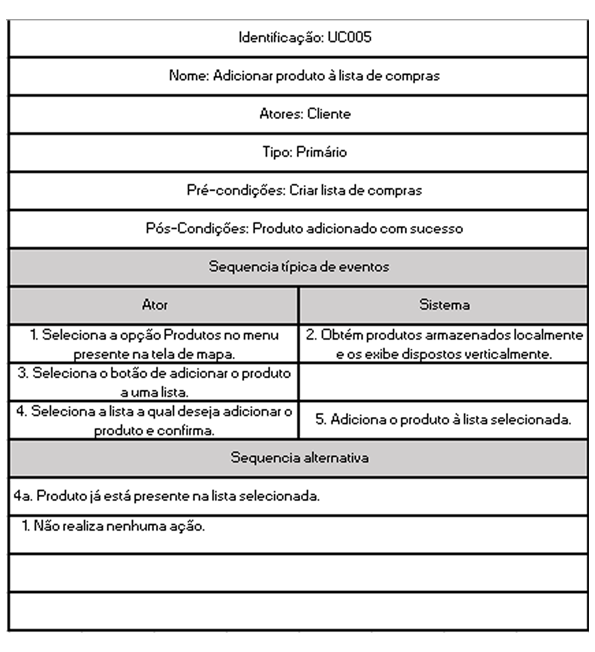
\includegraphics[scale=0.8]{Imagens/UC005.PNG}
		\fonte{Do autor - 2019.}
\end{figure}

\begin{figure}[H]
	\centering
		\caption{UC006}
		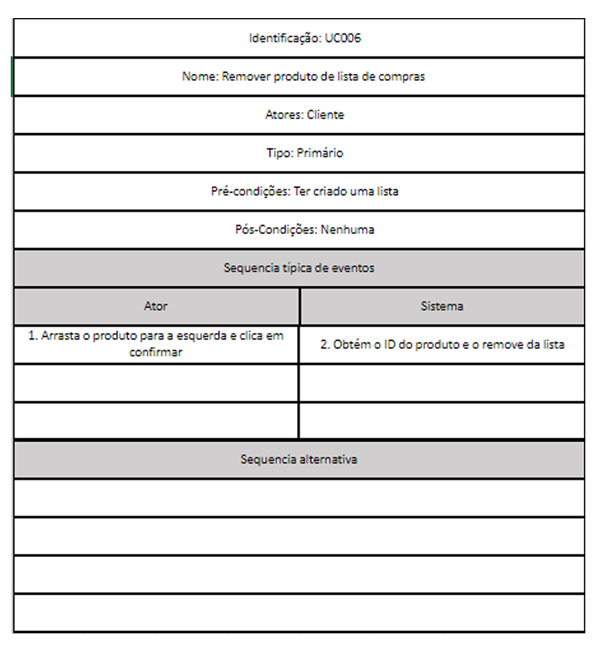
\includegraphics[scale=0.8]{Imagens/UC006.PNG}
		\fonte{Do autor - 2019.}
\end{figure}

\begin{figure}[H]
	\centering
		\caption{UC007}
		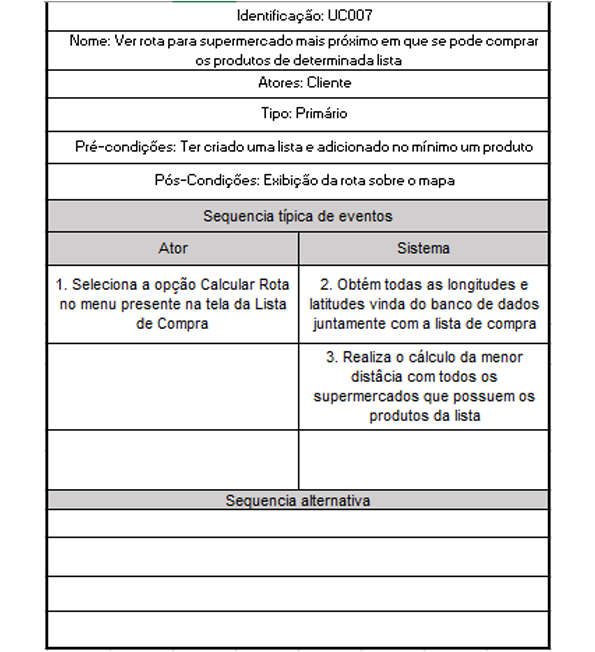
\includegraphics[scale=0.8]{Imagens/UC007.PNG}
		\fonte{Do autor - 2019.}
\end{figure}
	
\begin{figure}[H]
	\centering
		\caption{UC008}
		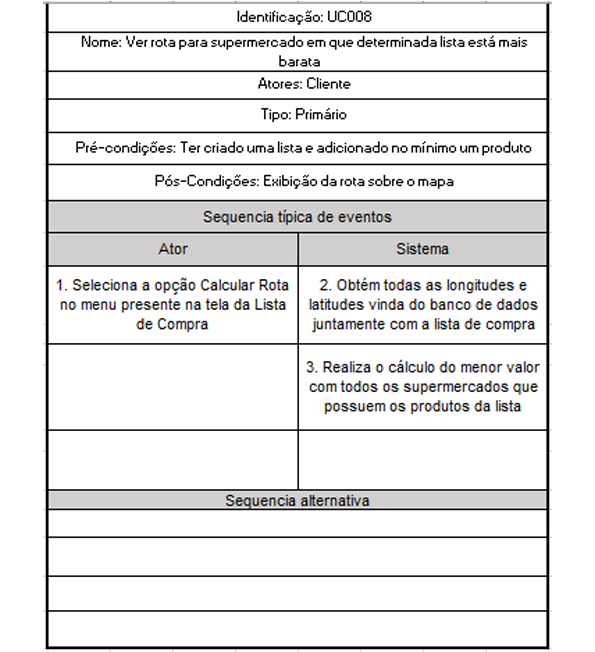
\includegraphics[scale=0.8]{Imagens/UC008.PNG}
		\fonte{Do autor - 2019.}
\end{figure}
	
\begin{figure}[H]
	\centering
		\caption{UC009}
		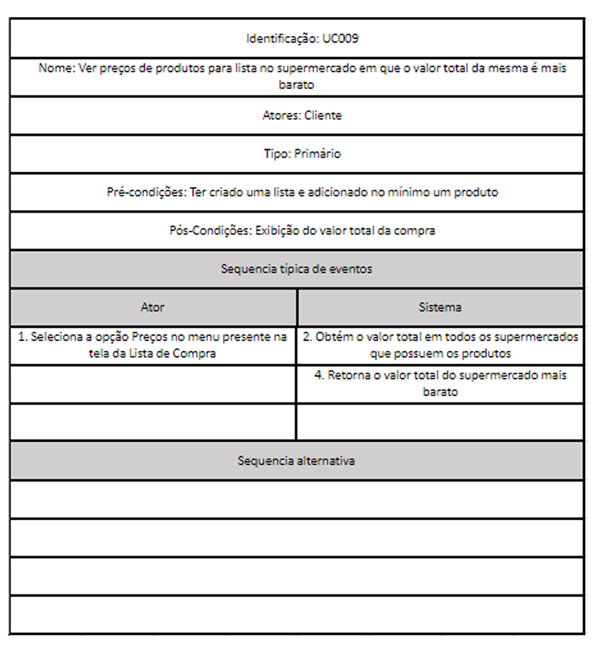
\includegraphics[scale=0.8]{Imagens/UC009.PNG}
		\fonte{Do autor - 2019.}
\end{figure}
	
\begin{figure}[H]
	\centering
		\caption{UC010}
		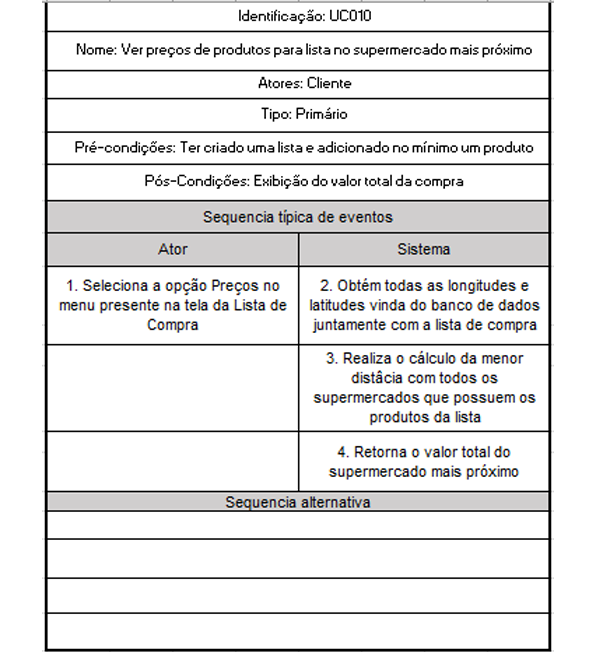
\includegraphics[scale=0.8]{Imagens/UC010.PNG}
		\fonte{Do autor - 2019.}
		\label{fig:UC010}	
\end{figure}


\section{Diagrama de atividades}
	Faz-se necessário descrever o algoritmo de forma bem explícita, e para tal, foi utilizado um diagrama de atividades, como vemos na figura \ref{fig:fluxograma}, o qual descreve sequência operacional das ações e tomadas de decisões que o usuário pode realizar no aplicativo.
	
\begin{figure}[H]
	\centering
		\caption{Diagrama de atividades do aplicativo Superbuscado}
		\includegraphics[scale=0.3]{Imagens/fluxograma.PNG}
		\fonte{Do autor - 2019.}
		\label{fig:fluxograma}	
\end{figure}

\section{Análise de requisitos}
\begin{itemize}
\item [RF001] O usuário deve ser capaz de visualizar no mapa os supermercados identificados com um marcador.
\item [RF002] O usuário deve ser capaz ver a lista dos produtos cadastrados, cada qual com nome, foto, categorias e preços, além de poder pesquisa-los pelo nome.
\item [RF003] O usuário deve ser capaz de criar e apagar listas de compras.
\item [RF004] O usuário deve ser capaz de adicionar e remover produtos de listas de compras.
\item [RF005] O usuário deve ser capaz de visualizar todos os produtos contidos em uma determinada lista de compras.
\item [RF006] O usuário deve ser capaz de visualizar a lista de compras feita tanto no supermercado em que ela se encontra mais barata quanto naquele em que a distância de deslocamento até o estabelecimento for menor.
\item [RF007] O usuário deve ser capaz de ver tanto a rota para o supermercado em que determinada lista de compras possui seu menor preço quanto para a rota direcionada para o supermercado com menor distância de deslocamento.
\end{itemize}

\begin{itemize}
\item [RNF001] O aplicativo não deve permitir a utilização com o GPS desligado.
\item [RNF002] O aplicativo deve manter suas telas atualizadas quando ocorrerem mudanças nos dados.
\item [RNF003] O aplicativo não deve sobrepor a menor rota no mapa com a rota mais barata.
\end{itemize}


\section{Análise de dados}
Para testar o desempenho do aplicativo, foram realizadas diversas possibilidades com rotas e quantidades de produtos, os resultados obtidos podem ser analisados na figura \ref{fig:tabelaestado}. Para tal teste, foram utilizados um Motorola Moto One Zoom (Processador: 8 core 1.8 GHZ, 3GB de RAM) e Xiaomi Redmi Note 7 (Processador: 8 core 2.0 GHZ, 3GB de RAM).

\begin{figure}[H]
   	\centering
   		\caption{Testes nos celulares Motorola Moto One Zoom e Xiaomi Redmi Note 7.}
	   	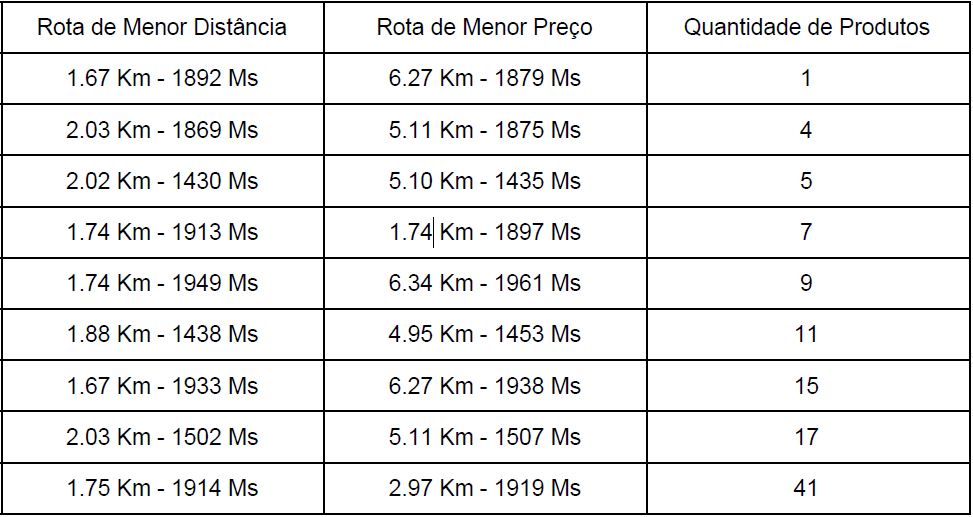
\includegraphics[scale=0.64]{Imagens/AnaliseDeDados.PNG}
   		\fonte{Do autor - 2019}
   		\label{fig:tabelaestado}
\end{figure}

Após uma análise profunda da performance no procedimento de cálculo de rota, notamos que o
tempo de execução é basicamente o mesmo independente da distância e do número de
produtos. Foi constatado também que a média do tempo de execução dos cálculos da menor
rota e da rota mais barata foram executados com tempos médios semelhantes. Baseando-se
nesses fatos, pode-se concluir que a complexidade de tempo de ambos pode ser considerada
a mesma levando em conta uma pequena margem de erro.

\begin{itemize}
\item Nos testes a média aritmética da menor distância foi de 1760 Ms.
\item Nos testes a média aritmética do menor preço foi de 1763 Ms.
\end{itemize}


\section{Documentação do banco de dados}
\subsection{Requisitos e regras de negócio}

\subsection{Estado}
	Entidade de unidades federativas, as quais fazem parte do endereço de um supermercado, o nome de estado é obrigatório e nunca irá se repetir, já que não existe mais de um estado com mesmo nome em um país.
	
\subsection{Cidade}
	Entidade cidades dos supermercados, várias cidades podem pertencer a um estado, mas uma cidade só pertence a um estado ao mesmo tempo, um nome de cidade pode existir em outro estado (nesse caso, cada cidade será tratada de forma diferente, de forma exclusiva), mas nunca poderá existir mais de uma cidade com mesmo nome em um único estado. Cada cidade deve obrigatoriamente ter um nome e estado.

\subsection{Bairro}
	Entidade de bairro dos supermercados, uma cidade pode ter vários bairros, mas um bairro só pode pertencer a uma cidade ao mesmo tempo, não pode haver bairros com mesmo nome em uma cidade, mas em outra cidade poderá ser aceito (nesse caso, cada bairro será tratado de forma diferente, como único). Todo bairro deverá ter nome, e uma cidade a ele relacionada, bem como uma cidade tem um estado. 

\subsection{Supermercado}
	Supermercado deve ter um bairro, que por sua vez deve ter uma cidade e essa ter um estado. Em um bairro pode haver diversos supermercados. Pode haver repetições de nomes de supermercados, porém cada um destes será tratado de forma diferente, como único. Cada supermercado deverá ter obrigatoriamente um nome, logradouro, bairro, latitude, longitude, opcionalmente pode ter um site.

\subsection{Produto}
	Cada produto deve ter nome único, não se pode repetir o nome deste, o produto deve pertencer a uma categoria ou mais de uma ao mesmo tempo, este pode estar em diversos supermercados ou em nenhum, ao passo que um supermercado pode ter diversos produtos. 

\subsection{Categoria}
	Uma categoria pode ter diversos produtos ou nenhum, não é permitido existir mais de uma categoria com mesmo nome.
	
\section{Dicionário de dados}
	Um dicionário de dados é fundamental em uma modelagem de banco de dados, sendo este utilizado para armazenar informações sobre o conteúdo, formato e estrutura de um banco de dados. Pode-se dizer que, um dicionário de dados são metadados, já que são dados de outros dados. Tendo em vista o grande potencial deste em uma documentação, segue abaixo (nas figuras \ref{fig:tabelaestado} a \ref{fig:tabelacamposunicos}) o dicionário de dados que tem como objetivo documentar o banco de dados usado no aplicativo.
	
\begin{figure}[H]
	\centering
	\caption{Tabela Estado.}
	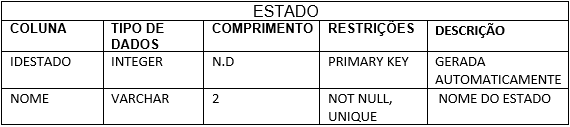
\includegraphics[scale=0.64]{Imagens/TabelaEstado.PNG}
	\fonte{Do autor - 2019}
    \label{fig:tabelaestado}
\end{figure}
						
\begin{figure}[H]
	\centering
    \caption{Tabela Cidade.}
    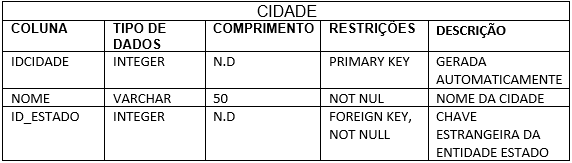
\includegraphics[scale=0.64]{Imagens/TabelaCidade.PNG}
    \fonte{Do autor - 2019}
\end{figure}
			
\begin{figure}[H]
    \centering
    \caption{Tabela Bairro.}
   	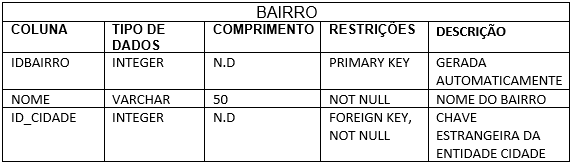
\includegraphics[scale=0.64]{Imagens/TabelaBairro.PNG}
  	\fonte{Do autor - 2019}
\end{figure}
			
\begin{figure}[H]
	\centering
    \caption{Tabela Supermercado.}
    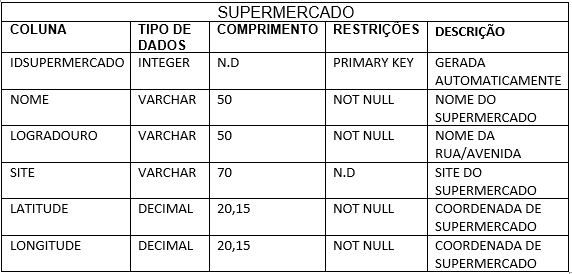
\includegraphics[scale=0.64]{Imagens/TabelaSupermercado.PNG}
    \fonte{Do autor - 2019}
\end{figure}
			
\begin{figure}[H]
    \centering
    \caption{Tabela Supermercado-Bairro.}
    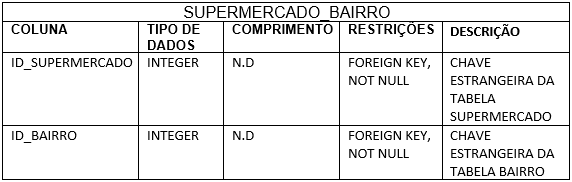
\includegraphics[scale=0.64]{Imagens/TabelaSupermercadoBairro.PNG}
    \fonte{Do autor - 2019}
\end{figure}
			
\begin{figure}[H]
    \centering
    \caption{Tabela Produto.}
    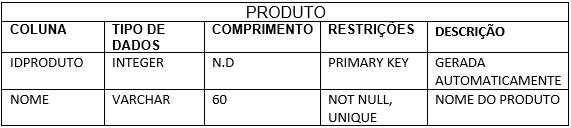
\includegraphics[scale=0.64]{Imagens/TabelaProduto.PNG}
    \fonte{Do autor - 2019}
\end{figure}
			
\begin{figure}[H]
    \centering
    \caption{Tabela Categoria.}
    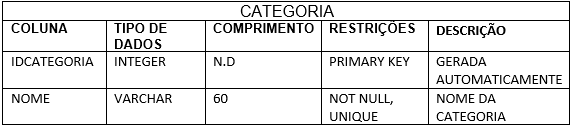
\includegraphics[scale=0.64]{Imagens/TabelaCategoria.PNG}
    \fonte{Do autor - 2019}
\end{figure}
			
\begin{figure}[H]
	\centering
	\caption{Tabela Produto-Categoria.}
	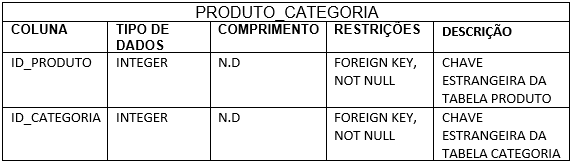
\includegraphics[scale=0.64]{Imagens/TabelaProdutoCategoria.PNG}
	\fonte{Do autor - 2019}
\end{figure}
			
\begin{figure}[H]
	\centering
    \caption{Tabela Supermercado-Produto.}
    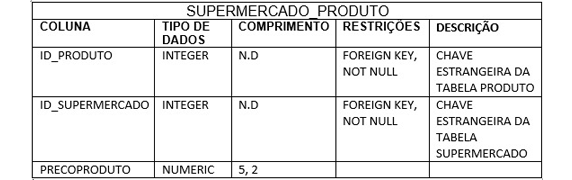
\includegraphics[scale=0.64]{Imagens/TabelaSupermercadoProduto.PNG}
    \fonte{Do autor - 2019}
\end{figure}
			
\begin{figure}[H]
	\centering
   	\caption{Tabela Chaves primárias.}
   	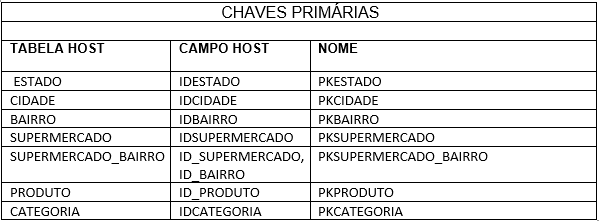
\includegraphics[scale=0.64]{Imagens/TabelaChavesPrimarias.PNG}
   	\fonte{Do autor - 2019}
\end{figure}
			
\begin{figure}[H]
  	\centering
   	\caption{Tabela Chaves estrangeiras.}
   	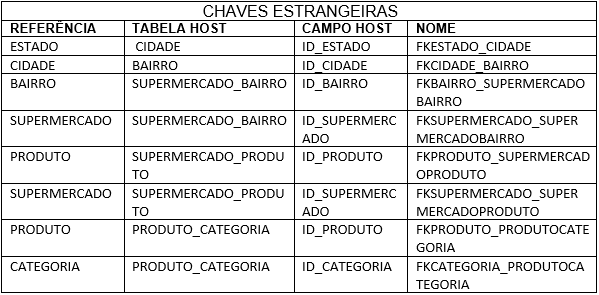
\includegraphics[scale=0.64]{Imagens/TabelaChavesEstrangeiras.PNG}
   	\fonte{Do autor - 2019}
\end{figure}
			
\begin{figure}[H]
  	\centering
   	\caption{Tabela Campos únicos.}
   	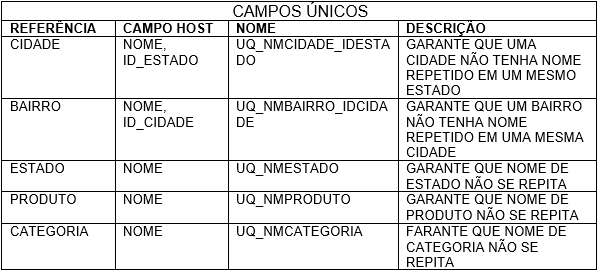
\includegraphics[scale=0.64]{Imagens/TabelaCamposUnicos.PNG}
   	\fonte{Do autor - 2019.}
   	\label{fig:tabelacamposunicos}
\end{figure}
		

\section{Modelagem lógica}
	A modelagem lógica possui o detalhamento da base de dados, de forma que o usuário possa entender facilmente toda a proposta do projeto. É um nível independente de SGBD, seu objetivo visa detalhar o banco de dados tanto para desenvolvedores de banco de dados quanto para os não desenvolvedores. Estão descritas na figura \ref{fig:modelagemlogica} tais representações.
	
\begin{figure}[H]
   	\centering
   	\caption{Modelagem Lógica.}
   	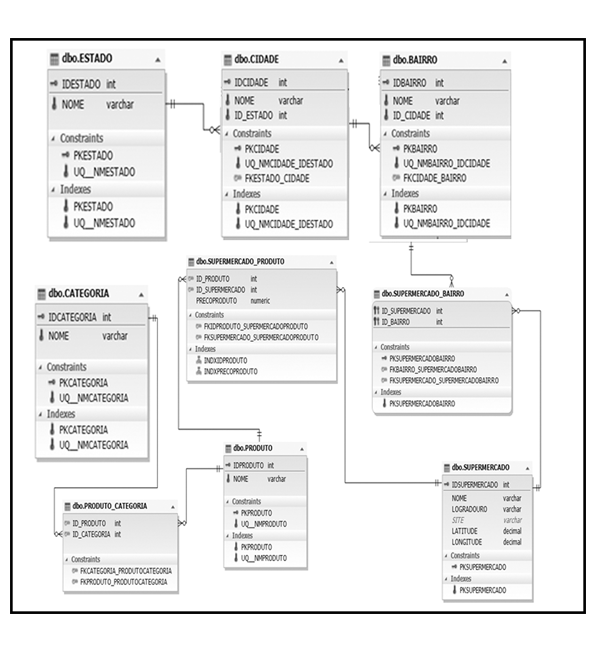
\includegraphics[scale=0.8]{Imagens/ModelagemLogica.png}
   	\fonte{Do autor - 2019.}
   	\label{fig:modelagemlogica}
\end{figure}
	
\section{Modelagem física}
	A modelagem física é o último passo na criação de um banco de dados, tal nível de modelagem depende do SGBD, tendo esses suas peculiaridades e algumas diferenças entre si. Este é o nível mais próximo entre homem e máquina no que se refere a banco de dados, não tem como objetivo detalhar o projeto para usuários, são de fato, scripts para serem processados por máquina, como nas figuras \ref{fig:modelagemfisica01} a \ref{fig:modelagemfisica03}.
	
\begin{figure}[H]
	\centering
	\caption{Modelagem Física - Imagem 01.}
	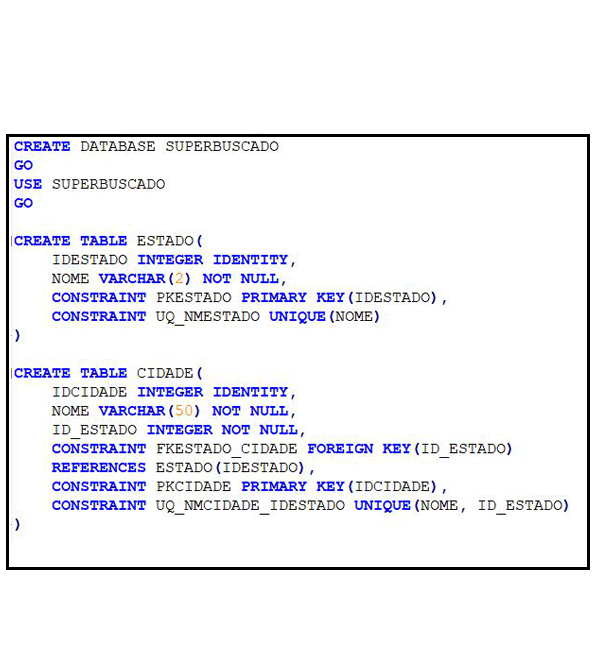
\includegraphics[scale=0.8]{Imagens/ModelagemFisica01.png}
	\fonte{Do autor - 2019.}
	\label{fig:modelagemfisica01}
\end{figure}
			
\begin{figure}[H]
	\centering
    \caption{Modelagem Física - Imagem 02.}
    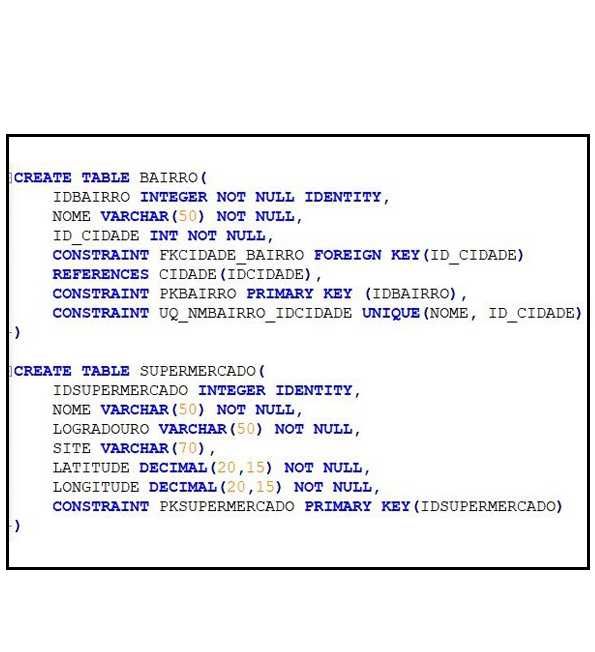
\includegraphics[scale=0.8]{Imagens/ModelagemFisica02.png}
    \fonte{Do autor - 2019.}
    \label{fig:modelagemfisica02}
\end{figure}
			
\begin{figure}[H]
   	\centering
    \caption{Modelagem Física - Imagem 03.}
    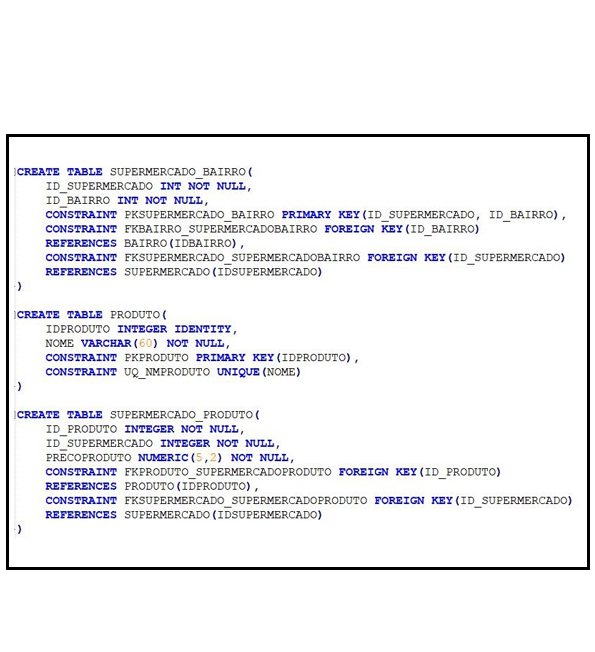
\includegraphics[scale=0.8]{Imagens/ModelagemFisica03.png}
    \fonte{Do autor - 2019.}
\end{figure}

\begin{figure}[H]
   	\centering
    \caption{Modelagem Física - Imagem 04.}
    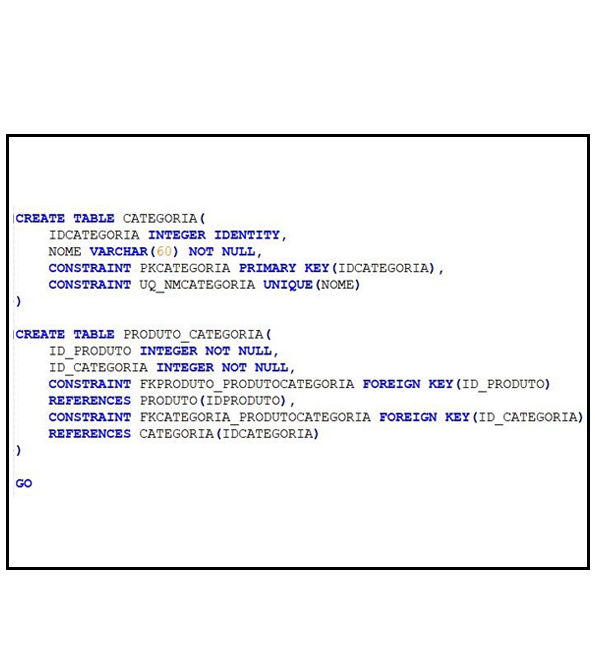
\includegraphics[scale=0.8]{Imagens/ModelagemFisica04.png}
    \fonte{Do autor - 2019.}
\end{figure}

			
\section{Criação de Views}
\begin{figure}[H]
    \centering
    \caption{Criação de Views - Imagem 01.}
    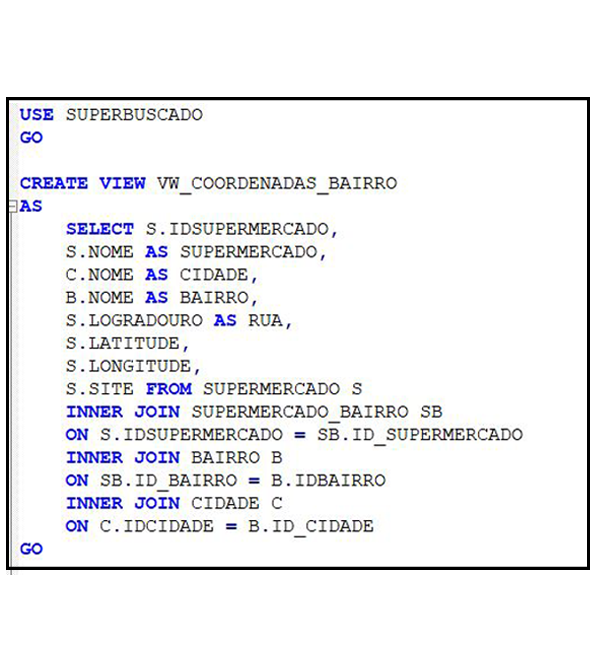
\includegraphics[scale=0.8]{Imagens/CriacaoDeViews01.png}
    \fonte{Do autor - 2019.}
\end{figure}

\begin{figure}[H]
	\centering
   	\caption{Criação de Views - Imagem 02.}
   	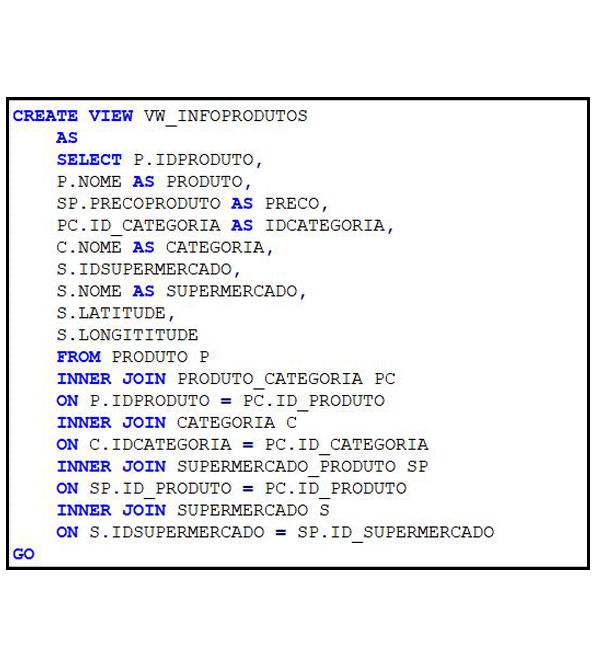
\includegraphics[scale=0.8]{Imagens/CriacaoDeViews02.png}
   	\fonte{Do autor - 2019.}
   	\label{fig:modelagemfisica03}
\end{figure}
			
\subsection{Diagrama de visões}
	\begin{figure}[H]
    \centering
    \caption{Diagrama.}
    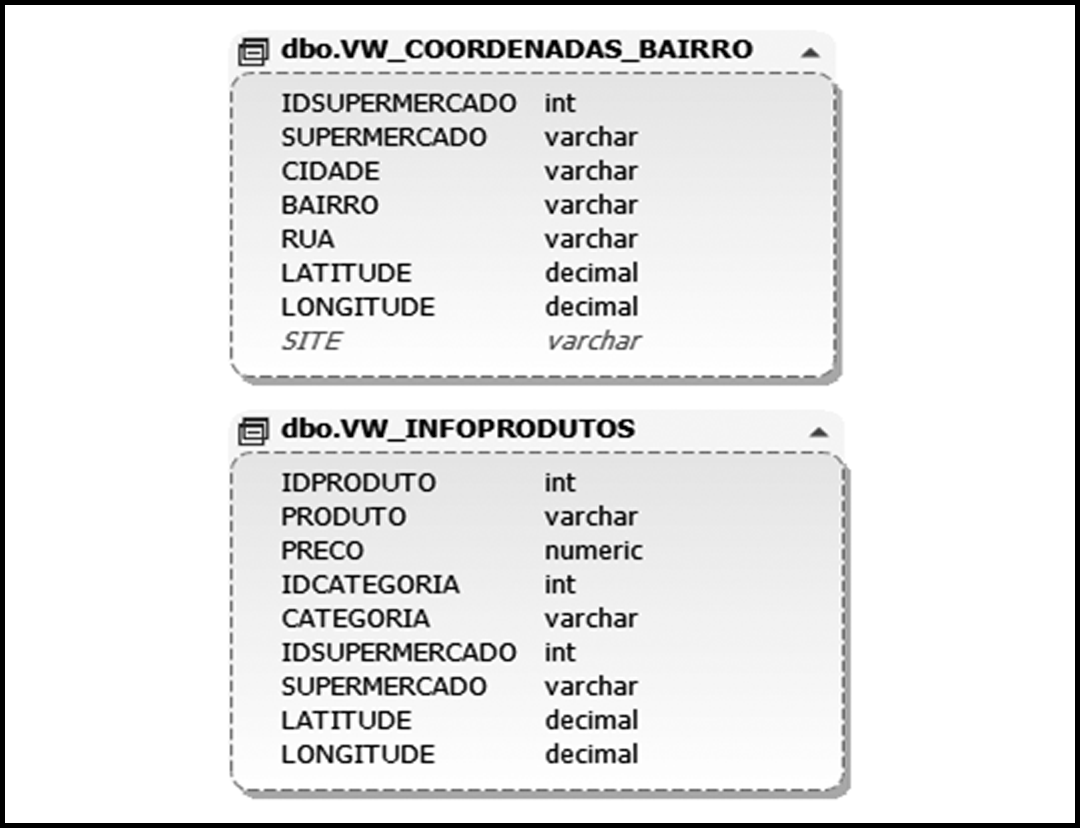
\includegraphics[scale=0.3]{Imagens/ViewsDiagrama.png}
    \fonte{Do autor - 2019.}
\end{figure}

\section{Interface do aplicativo}
Está é a tela inicial da aplicação, começa na área do GPS para garantir que logo no começo do uso todos os itens necessários estejam ativos, além de ser uma funcionalidade a mais, pois assim o usuário pode apenas consultar um caminho para um supermercado específico caso o queira.
\begin{figure}[H]
    \centering
    \caption{Tela Inicial.}
    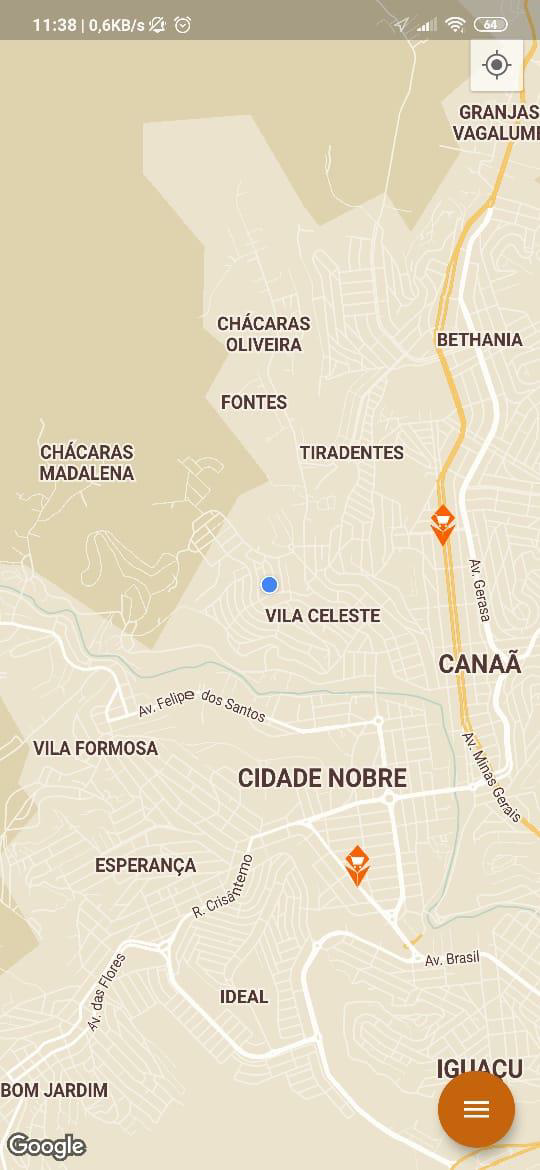
\includegraphics[scale=0.3]{Imagens/Print01.png}
    \fonte{Do autor - 2019.}
\end{figure}

Clicando no Menu no canto inferior direito, irá aparecer duas opções: “Produtos” e “Lista de Compras”.
\begin{figure}[H]
    \centering
    \caption{Tela Menu inferior.}
    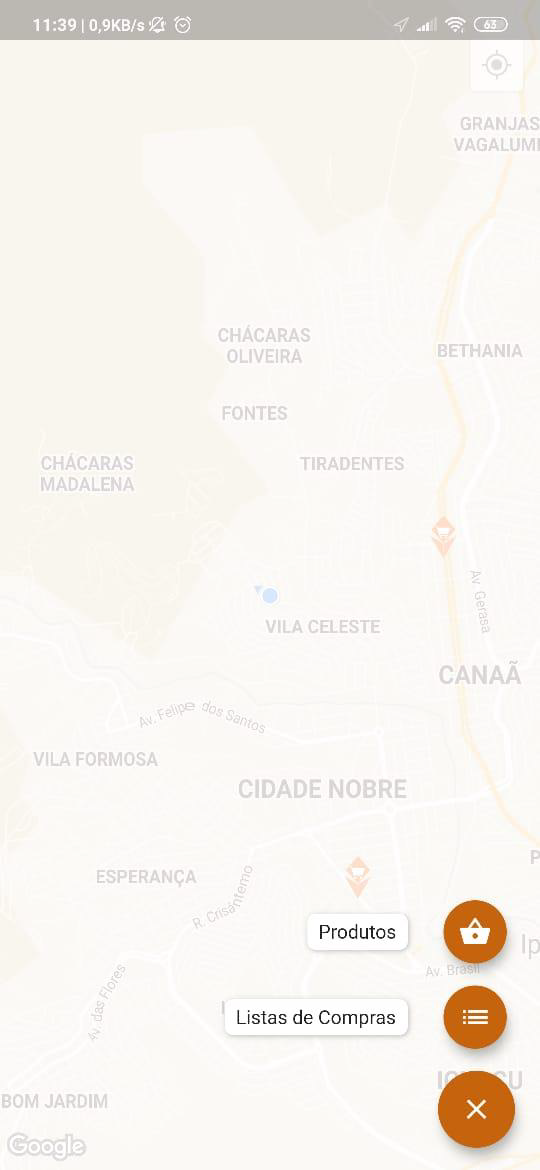
\includegraphics[scale=0.3]{Imagens/Print02.png}
    \fonte{Do autor - 2019.}
\end{figure}


Ao clicar em “Produtos” irá aparecer uma lista de todos os produtos cadastrados em nosso banco de dados. Arrastando o nome do produto para o lado direito aparecerá à imagem referente aquele produto em específico. Para retirar basta arrastar para o lado esquerdo.
\begin{figure}[H]
    \centering
    \caption{Tela Produtos.}
    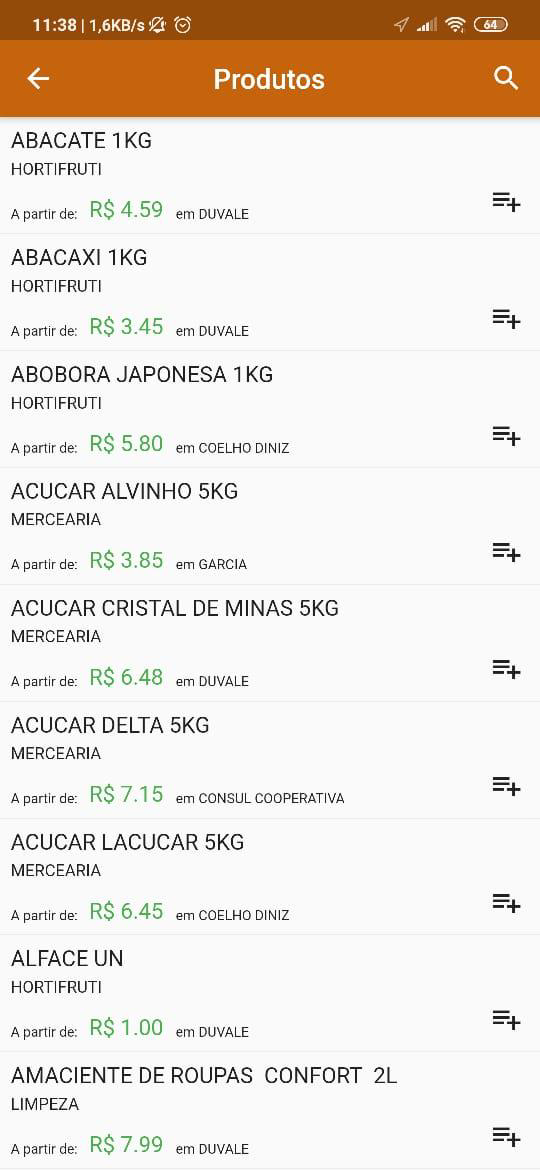
\includegraphics[scale=0.3]{Imagens/Print03.png}
    \fonte{Do autor - 2019.}
\end{figure}


Para adicionar um produto à lista basta clicar no símbolo à direita do mesmo, caso não tenha nenhuma lista cadastrada basta clicar em “Nova Lista”. Após nomear à lista basta confirmar e o item será adicionado.
\begin{figure}[H]
    \centering
    \caption{Tela Nova lista.}
    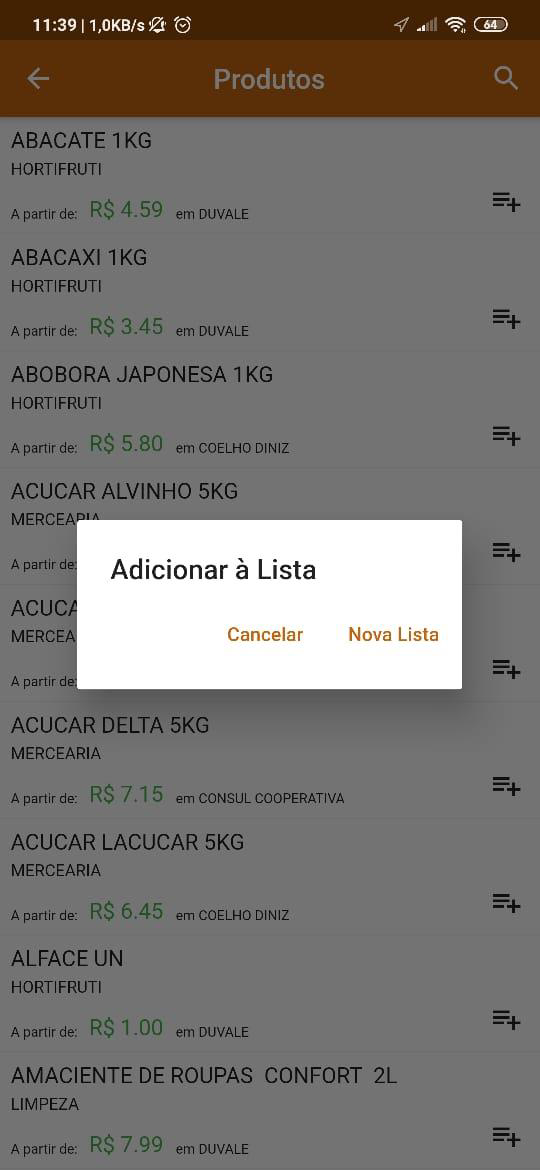
\includegraphics[scale=0.3]{Imagens/Print04.png}
    \fonte{Do autor - 2019.}
\end{figure}


Ao clicar em “Listas de Compras”, irão aparecer todas as listas já criadas com o número de produtos de cada lista.
\begin{figure}[H]
    \centering
    \caption{Tela Lista de compras.}
    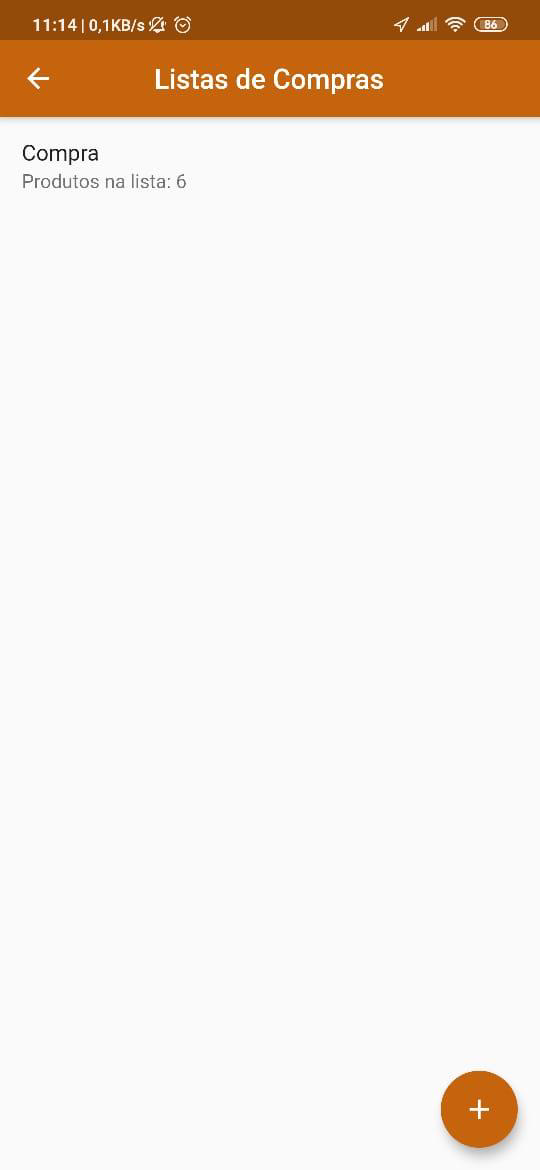
\includegraphics[scale=0.3]{Imagens/Print05.png}
    \fonte{Do autor - 2019.}
\end{figure}


Após selecionar uma lista vai aparecer um Menu com três opções: “Preços”, “Calcular Rota” e “Adicionar Produtos”. Ao selecionar “Preços” à aplicação retornará um ou dois valores. Se existir somente um valor significa que o local mais perto também é o mais barato, caso retorne dois valores, o da esquerda será o mais barato e o da direito o mais perto.
\begin{figure}[H]
    \centering
    \caption{Tela Menu de opções.}
    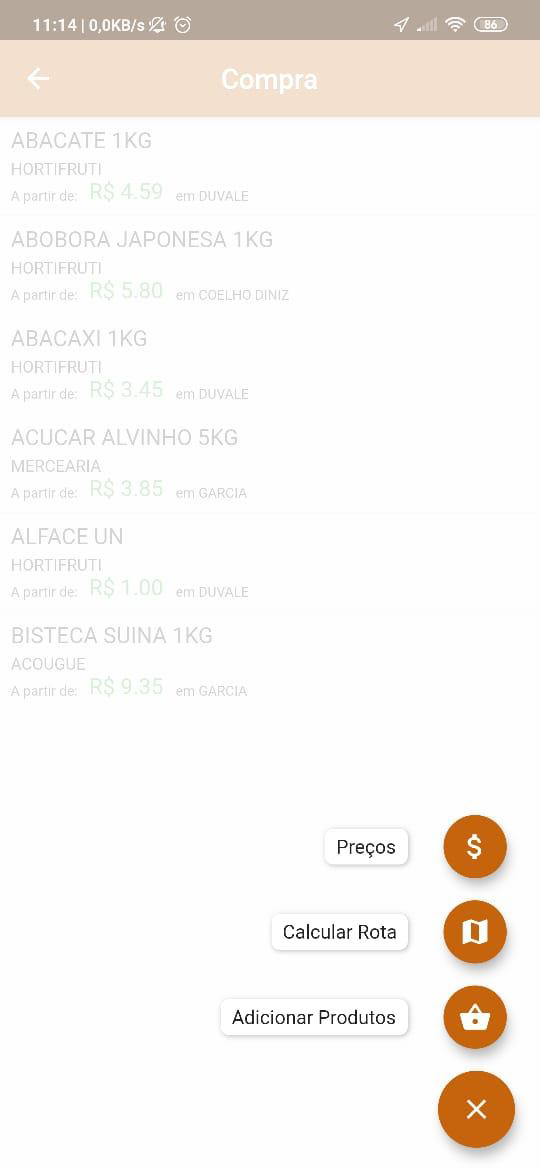
\includegraphics[scale=0.3]{Imagens/Print06.png}
    \fonte{Do autor - 2019.}
\end{figure}


Selecionando a opção “Rotas” o aplicativo estará mostrando a rota tanto do mais próximo quanto do mais barato. Ao clicar na opção desejada, a cor irá sobrepor a que não foi selecionada, podendo ser trocada em tempo de execução.
\begin{figure}[H]
    \centering
    \caption{Tela Rotas.}
    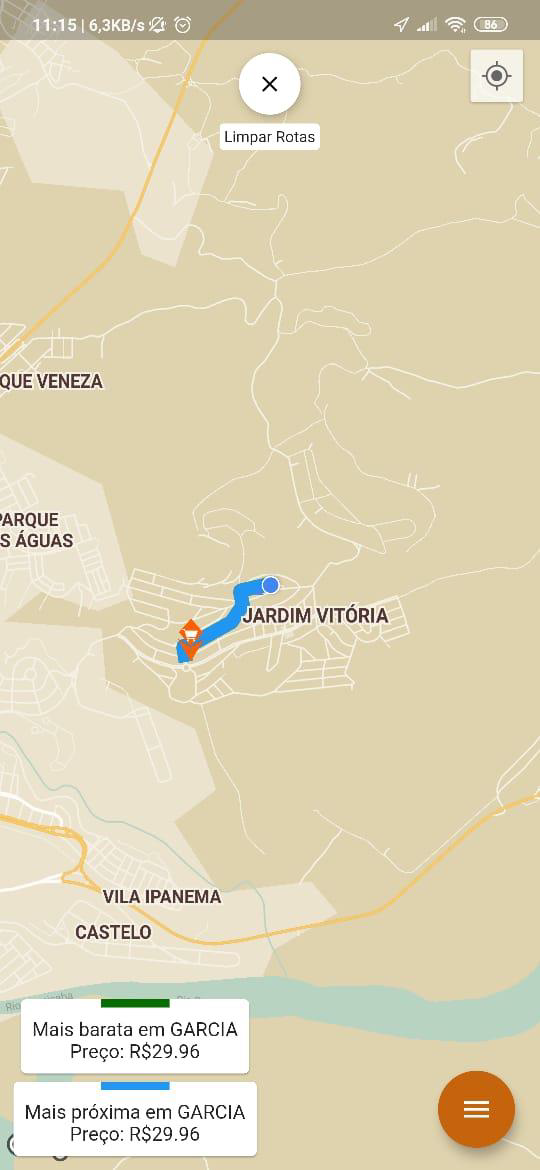
\includegraphics[scale=0.3]{Imagens/Print07.png}
    \fonte{Do autor - 2019.}
\end{figure}